%%%%%%%%%%%%%%%%%%%%%%%%%%%%%%%%%%%%%%%%%
% The Legrand Orange Book
% LaTeX Template
% Version 2.0 (9/2/15)
%
% This template has been downloaded from:
% http://www.LaTeXTemplates.com
%
% Mathias Legrand (legrand.mathias@gmail.com) with modifications by:
% Vel (vel@latextemplates.com)
%
% License:
% CC BY-NC-SA 3.0 (http://creativecommons.org/licenses/by-nc-sa/3.0/)
%
% Compiling this template:
% This template uses biber for its bibliography and makeindex for its index.
% When you first open the template, compile it from the command line with the
% commands below to make sure your LaTeX distribution is configured correctly:
%
% 1) pdflatex main
% 2) makeindex main.idx -s StyleInd.ist
% 3) biber main
% 4) pdflatex main x 2
%
% After this, when you wish to update the bibliography/index use the appropriate
% command above and make sure to compile with pdflatex several times
% afterwards to propagate your changes to the document.
%
% This template also uses a number of packages which may need to be
% updated to the newest versions for the template to compile. It is strongly
% recommended you update your LaTeX distribution if you have any
% compilation errors.
%
% Important note:
% Chapter heading images should have a 2:1 width:height ratio,
% e.g. 920px width and 460px height.
%
%%%%%%%%%%%%%%%%%%%%%%%%%%%%%%%%%%%%%%%%%

%----------------------------------------------------------------------------------------
%	PACKAGES AND OTHER DOCUMENT CONFIGURATIONS
%----------------------------------------------------------------------------------------

\documentclass[12pt,fleqn]{book} % Default font size and left-justified equations

%----------------------------------------------------------------------------------------

%%%%%%%%%%%%%%%%%%%%%%%%%%%%%%%%%%%%%%%%%
% The Legrand Orange Book
% Structural Definitions File
% Version 2.0 (9/2/15)
%
% Original author:
% Mathias Legrand (legrand.mathias@gmail.com) with modifications by:
% Vel (vel@latextemplates.com)
%
% This file has been downloaded from:
% http://www.LaTeXTemplates.com
%
% License:
% CC BY-NC-SA 3.0 (http://creativecommons.org/licenses/by-nc-sa/3.0/)
%
%%%%%%%%%%%%%%%%%%%%%%%%%%%%%%%%%%%%%%%%%

%----------------------------------------------------------------------------------------
%	VARIOUS REQUIRED PACKAGES AND CONFIGURATIONS
%----------------------------------------------------------------------------------------

\usepackage[top=3cm,bottom=3cm,left=3cm,right=3cm,headsep=10pt,a4paper]{geometry} % Page margins

\usepackage{graphicx} % Required for including pictures
\graphicspath{{pictures/}} % Specifies the directory where pictures are stored

\usepackage{lipsum} % Inserts dummy text

\usepackage{tikz} % Required for drawing custom shapes

\usepackage[english]{babel} % English language/hyphenation

\usepackage{enumitem} % Customize lists
\setlist{nolistsep} % Reduce spacing between bullet points and numbered lists

\usepackage{booktabs} % Required for nicer horizontal rules in tables

\usepackage{xcolor,colortbl} % Required for specifying colors by name
%\definecolor{ocre}{RGB}{243,102,25} % Define the orange color used for highlighting throughout the book
\definecolor{ocre}{RGB}{0,0,51}

%----------------------------------------------------------------------------------------
%	FONTS
%----------------------------------------------------------------------------------------

\usepackage{avant} % Use the Avantgarde font for headings
%\usepackage{times} % Use the Times font for headings
\usepackage{mathptmx} % Use the Adobe Times Roman as the default text font together with math symbols from the Sym­bol, Chancery and Com­puter Modern fonts

\usepackage{microtype} % Slightly tweak font spacing for aesthetics
\usepackage[utf8]{inputenc} % Required for including letters with accents
\usepackage[T1]{fontenc} % Use 8-bit encoding that has 256 glyphs

%----------------------------------------------------------------------------------------
%	BIBLIOGRAPHY AND INDEX
%----------------------------------------------------------------------------------------

\usepackage[style=alphabetic,citestyle=numeric,sorting=nyt,sortcites=true,autopunct=true,babel=hyphen,hyperref=true,abbreviate=false,backref=true,backend=biber]{biblatex}
\addbibresource{bibliography.bib} % BibTeX bibliography file
\defbibheading{bibempty}{}

\usepackage{calc} % For simpler calculation - used for spacing the index letter headings correctly
\usepackage{makeidx} % Required to make an index
\makeindex % Tells LaTeX to create the files required for indexing

%----------------------------------------------------------------------------------------
%	MAIN TABLE OF CONTENTS
%----------------------------------------------------------------------------------------

\usepackage{titletoc} % Required for manipulating the table of contents

\contentsmargin{0cm} % Removes the default margin

% Part text styling
\titlecontents{part}[0cm]
{\addvspace{20pt}\centering\large\bfseries}
{}
{}
{}

% Chapter text styling
\titlecontents{chapter}[1.25cm] % Indentation
{\addvspace{12pt}\large\sffamily\bfseries} % Spacing and font options for chapters
{\color{ocre!60}\contentslabel[\Large\thecontentslabel]{1.25cm}\color{ocre}} % Chapter number
{\color{ocre}}
{\color{ocre!60}\normalsize\;\titlerule*[.5pc]{.}\;\thecontentspage} % Page number

% Section text styling
\titlecontents{section}[1.25cm] % Indentation
{\addvspace{3pt}\sffamily\bfseries} % Spacing and font options for sections
{\contentslabel[\thecontentslabel]{1.25cm}} % Section number
{}
{\hfill\color{black}\thecontentspage} % Page number
[]

% Subsection text styling
\titlecontents{subsection}[1.25cm] % Indentation
{\addvspace{1pt}\sffamily\small} % Spacing and font options for subsections
{\contentslabel[\thecontentslabel]{1.25cm}} % Subsection number
{}
{\ \titlerule*[.5pc]{.}\;\thecontentspage} % Page number
[]

% List of figures
\titlecontents{figure}[0em]
{\addvspace{-5pt}\sffamily}
{\thecontentslabel\hspace*{1em}}
{}
{\ \titlerule*[.5pc]{.}\;\thecontentspage}
[]

% List of tables
\titlecontents{table}[0em]
{\addvspace{-5pt}\sffamily}
{\thecontentslabel\hspace*{1em}}
{}
{\ \titlerule*[.5pc]{.}\;\thecontentspage}
[]

%----------------------------------------------------------------------------------------
%	MINI TABLE OF CONTENTS IN PART HEADS
%----------------------------------------------------------------------------------------

% Chapter text styling
\titlecontents{lchapter}[0em] % Indenting
{\addvspace{15pt}\large\sffamily\bfseries} % Spacing and font options for chapters
{\color{ocre}\contentslabel[\Large\thecontentslabel]{1.25cm}\color{ocre}} % Chapter number
{}
{\color{ocre}\normalsize\sffamily\bfseries\;\titlerule*[.5pc]{.}\;\thecontentspage} % Page number

% Section text styling
\titlecontents{lsection}[0em] % Indenting
{\sffamily\small} % Spacing and font options for sections
{\contentslabel[\thecontentslabel]{1.25cm}} % Section number
{}
{}

% Subsection text styling
\titlecontents{lsubsection}[.5em] % Indentation
{\normalfont\footnotesize\sffamily} % Font settings
{}
{}
{}

%----------------------------------------------------------------------------------------
%	PAGE HEADERS
%----------------------------------------------------------------------------------------

\usepackage{fancyhdr} % Required for header and footer configuration

\pagestyle{fancy}
\renewcommand{\chaptermark}[1]{\markboth{\sffamily\normalsize\bfseries\chaptername\ \thechapter.\ #1}{}} % Chapter text font settings
\renewcommand{\sectionmark}[1]{\markright{\sffamily\normalsize\thesection\hspace{5pt}#1}{}} % Section text font settings
\fancyhf{} \fancyhead[LE,RO]{\sffamily\normalsize\thepage} % Font setting for the page number in the header
\fancyhead[LO]{\rightmark} % Print the nearest section name on the left side of odd pages
\fancyhead[RE]{\leftmark} % Print the current chapter name on the right side of even pages
\renewcommand{\headrulewidth}{0.5pt} % Width of the rule under the header
\addtolength{\headheight}{2.5pt} % Increase the spacing around the header slightly
\renewcommand{\footrulewidth}{0pt} % Removes the rule in the footer
\fancypagestyle{plain}{\fancyhead{}\renewcommand{\headrulewidth}{0pt}} % Style for when a plain pagestyle is specified

% Removes the header from odd empty pages at the end of chapters
\makeatletter
\renewcommand{\cleardoublepage}{
\clearpage\ifodd\c@page\else
\hbox{}
\vspace*{\fill}
\thispagestyle{empty}
\newpage
\fi}

%----------------------------------------------------------------------------------------
%	THEOREM STYLES
%----------------------------------------------------------------------------------------

\usepackage{amsmath,amsfonts,amssymb,amsthm} % For math equations, theorems, symbols, etc

\newcommand{\intoo}[2]{\mathopen{]}#1\,;#2\mathclose{[}}
\newcommand{\ud}{\mathop{\mathrm{{}d}}\mathopen{}}
\newcommand{\intff}[2]{\mathopen{[}#1\,;#2\mathclose{]}}
\newtheorem{notation}{Notation}[chapter]

% Boxed/framed environments
\newtheoremstyle{ocrenumbox}% % Theorem style name
{0pt}% Space above
{0pt}% Space below
{\normalfont}% % Body font
{}% Indent amount
{\small\bf\sffamily\color{ocre}}% % Theorem head font
{\;}% Punctuation after theorem head
{0.25em}% Space after theorem head
{\small\sffamily\color{ocre}\thmname{#1}\nobreakspace\thmnumber{\@ifnotempty{#1}{}\@upn{#2}}% Theorem text (e.g. Theorem 2.1)
\thmnote{\nobreakspace\the\thm@notefont\sffamily\bfseries\color{black}---\nobreakspace#3.}} % Optional theorem note
\renewcommand{\qedsymbol}{$\blacksquare$}% Optional qed square

\newtheoremstyle{blacknumex}% Theorem style name
{5pt}% Space above
{5pt}% Space below
{\normalfont}% Body font
{} % Indent amount
{\small\bf\sffamily}% Theorem head font
{\;}% Punctuation after theorem head
{0.25em}% Space after theorem head
{\small\sffamily{\tiny\ensuremath{\blacksquare}}\nobreakspace\thmname{#1}\nobreakspace\thmnumber{\@ifnotempty{#1}{}\@upn{#2}}% Theorem text (e.g. Theorem 2.1)
\thmnote{\nobreakspace\the\thm@notefont\sffamily\bfseries---\nobreakspace#3.}}% Optional theorem note

\newtheoremstyle{blacknumbox} % Theorem style name
{0pt}% Space above
{0pt}% Space below
{\normalfont}% Body font
{}% Indent amount
{\small\bf\sffamily}% Theorem head font
{\;}% Punctuation after theorem head
{0.25em}% Space after theorem head
{\small\sffamily\thmname{#1}\nobreakspace\thmnumber{\@ifnotempty{#1}{}\@upn{#2}}% Theorem text (e.g. Theorem 2.1)
\thmnote{\nobreakspace\the\thm@notefont\sffamily\bfseries---\nobreakspace#3.}}% Optional theorem note

% Non-boxed/non-framed environments
\newtheoremstyle{ocrenum}% % Theorem style name
{5pt}% Space above
{5pt}% Space below
{\normalfont}% % Body font
{}% Indent amount
{\small\bf\sffamily\color{ocre}}% % Theorem head font
{\;}% Punctuation after theorem head
{0.25em}% Space after theorem head
{\small\sffamily\color{ocre}\thmname{#1}\nobreakspace\thmnumber{\@ifnotempty{#1}{}\@upn{#2}}% Theorem text (e.g. Theorem 2.1)
\thmnote{\nobreakspace\the\thm@notefont\sffamily\bfseries\color{black}---\nobreakspace#3.}} % Optional theorem note
\renewcommand{\qedsymbol}{$\blacksquare$}% Optional qed square
\makeatother

% Defines the theorem text style for each type of theorem to one of the three styles above
\newcounter{dummy}
\numberwithin{dummy}{section}
\theoremstyle{ocrenumbox}
\newtheorem{theoremeT}[dummy]{Theorem}
\newtheorem{problem}{Problem}[chapter]
\newtheorem{exerciseT}{Exercise}[chapter]
\theoremstyle{blacknumex}
\newtheorem{exampleT}{Example}[chapter]
\theoremstyle{blacknumbox}
\newtheorem{vocabulary}{Vocabulary}[chapter]
\newtheorem{definitionT}{Definition}[section]
\newtheorem{corollaryT}[dummy]{Corollary}
\theoremstyle{ocrenum}
\newtheorem{proposition}[dummy]{Proposition}

%----------------------------------------------------------------------------------------
%	DEFINITION OF COLORED BOXES
%----------------------------------------------------------------------------------------

\RequirePackage[framemethod=default]{mdframed} % Required for creating the theorem, definition, exercise and corollary boxes

% Theorem box
\newmdenv[skipabove=7pt,
skipbelow=7pt,
backgroundcolor=black!5,
linecolor=ocre,
innerleftmargin=5pt,
innerrightmargin=5pt,
innertopmargin=5pt,
leftmargin=0cm,
rightmargin=0cm,
innerbottommargin=5pt]{tBox}

% Exercise box
\newmdenv[skipabove=7pt,
skipbelow=7pt,
rightline=false,
leftline=true,
topline=false,
bottomline=false,
backgroundcolor=ocre!10,
linecolor=ocre,
innerleftmargin=5pt,
innerrightmargin=5pt,
innertopmargin=5pt,
innerbottommargin=5pt,
leftmargin=0cm,
rightmargin=0cm,
linewidth=4pt]{eBox}

% Definition box
\newmdenv[skipabove=7pt,
skipbelow=7pt,
rightline=false,
leftline=true,
topline=false,
bottomline=false,
linecolor=ocre,
innerleftmargin=5pt,
innerrightmargin=5pt,
innertopmargin=0pt,
leftmargin=0cm,
rightmargin=0cm,
linewidth=4pt,
innerbottommargin=0pt]{dBox}

% Corollary box
\newmdenv[skipabove=7pt,
skipbelow=7pt,
rightline=false,
leftline=true,
topline=false,
bottomline=false,
linecolor=gray,
backgroundcolor=black!5,
innerleftmargin=5pt,
innerrightmargin=5pt,
innertopmargin=5pt,
leftmargin=0cm,
rightmargin=0cm,
linewidth=4pt,
innerbottommargin=5pt]{cBox}

% Creates an environment for each type of theorem and assigns it a theorem text style from the "Theorem Styles" section above and a colored box from above
\newenvironment{theorem}{\begin{tBox}\begin{theoremeT}}{\end{theoremeT}\end{tBox}}
\newenvironment{exercise}{\begin{eBox}\begin{exerciseT}}{\hfill{\color{ocre}\tiny\ensuremath{\blacksquare}}\end{exerciseT}\end{eBox}}
\newenvironment{definition}{\begin{dBox}\begin{definitionT}}{\end{definitionT}\end{dBox}}
\newenvironment{example}{\begin{exampleT}}{\hfill{\tiny\ensuremath{\blacksquare}}\end{exampleT}}
\newenvironment{corollary}{\begin{cBox}\begin{corollaryT}}{\end{corollaryT}\end{cBox}}

%----------------------------------------------------------------------------------------
%	REMARK ENVIRONMENT
%----------------------------------------------------------------------------------------

\newenvironment{remark}{\par\vspace{10pt}\small % Vertical white space above the remark and smaller font size
\begin{list}{}{
\leftmargin=35pt % Indentation on the left
\rightmargin=25pt}\item\ignorespaces % Indentation on the right
\makebox[-2.5pt]{\begin{tikzpicture}[overlay]
\node[draw=ocre!60,line width=1pt,circle,fill=ocre!25,font=\sffamily\bfseries,inner sep=2pt,outer sep=0pt] at (-15pt,0pt){\textcolor{ocre}{R}};\end{tikzpicture}} % Orange R in a circle
\advance\baselineskip -1pt}{\end{list}\vskip5pt} % Tighter line spacing and white space after remark

%----------------------------------------------------------------------------------------
%	SECTION NUMBERING IN THE MARGIN
%----------------------------------------------------------------------------------------

\makeatletter
\renewcommand{\@seccntformat}[1]{\llap{\textcolor{ocre}{\csname the#1\endcsname}\hspace{1em}}}
\renewcommand{\section}{\@startsection{section}{1}{\z@}
{-4ex \@plus -1ex \@minus -.4ex}
{1ex \@plus.2ex }
{\normalfont\large\sffamily\bfseries}}
\renewcommand{\subsection}{\@startsection {subsection}{2}{\z@}
{-3ex \@plus -0.1ex \@minus -.4ex}
{0.5ex \@plus.2ex }
{\normalfont\sffamily\bfseries}}
\renewcommand{\subsubsection}{\@startsection {subsubsection}{3}{\z@}
{-2ex \@plus -0.1ex \@minus -.2ex}
{.2ex \@plus.2ex }
{\normalfont\small\sffamily\bfseries}}
\renewcommand\paragraph{\@startsection{paragraph}{4}{\z@}
{-2ex \@plus-.2ex \@minus .2ex}
{.1ex}
{\normalfont\small\sffamily\bfseries}}

%----------------------------------------------------------------------------------------
%	PART HEADINGS
%----------------------------------------------------------------------------------------

% numbered part in the table of contents
\newcommand{\@mypartnumtocformat}[2]{%
\setlength\fboxsep{0pt}%
\noindent\colorbox{ocre!20}{\strut\parbox[c][.7cm]{\ecart}{\color{ocre!70}\Large\sffamily\bfseries\centering#1}}\hskip\esp\colorbox{ocre!40}{\strut\parbox[c][.7cm]{\linewidth-\ecart-\esp}{\Large\sffamily\centering#2}}}%
%%%%%%%%%%%%%%%%%%%%%%%%%%%%%%%%%%
% unnumbered part in the table of contents
\newcommand{\@myparttocformat}[1]{%
\setlength\fboxsep{0pt}%
\noindent\colorbox{ocre!40}{\strut\parbox[c][.7cm]{\linewidth}{\Large\sffamily\centering#1}}}%
%%%%%%%%%%%%%%%%%%%%%%%%%%%%%%%%%%
\newlength\esp
\setlength\esp{4pt}
\newlength\ecart
\setlength\ecart{1.2cm-\esp}
\newcommand{\thepartimage}{}%
\newcommand{\partimage}[1]{\renewcommand{\thepartimage}{#1}}%
\def\@part[#1]#2{%
\ifnum \c@secnumdepth >-2\relax%
\refstepcounter{part}%
\addcontentsline{toc}{part}{\texorpdfstring{\protect\@mypartnumtocformat{\thepart}{#1}}{\partname~\thepart\ ---\ #1}}
\else%
\addcontentsline{toc}{part}{\texorpdfstring{\protect\@myparttocformat{#1}}{#1}}%
\fi%
\startcontents%
\markboth{}{}%
{\thispagestyle{empty}%
\begin{tikzpicture}[remember picture,overlay]%
\node at (current page.north west){\begin{tikzpicture}[remember picture,overlay]%
\fill[ocre!20](0cm,0cm) rectangle (\paperwidth,-\paperheight);
\node[anchor=north] at (4cm,-3.25cm){\color{ocre!40}\fontsize{220}{100}\sffamily\bfseries\@Roman\c@part};
\node[anchor=south east] at (\paperwidth-1cm,-\paperheight+1cm){\parbox[t][][t]{8.5cm}{
\printcontents{l}{0}{\setcounter{tocdepth}{1}}%
}};
\node[anchor=north east] at (\paperwidth-1.5cm,-3.25cm){\parbox[t][][t]{15cm}{\strut\raggedleft\color{white}\fontsize{30}{30}\sffamily\bfseries#2}};
\end{tikzpicture}};
\end{tikzpicture}}%
\@endpart}
\def\@spart#1{%
\startcontents%
\phantomsection
{\thispagestyle{empty}%
\begin{tikzpicture}[remember picture,overlay]%
\node at (current page.north west){\begin{tikzpicture}[remember picture,overlay]%
\fill[ocre!20](0cm,0cm) rectangle (\paperwidth,-\paperheight);
\node[anchor=north east] at (\paperwidth-1.5cm,-3.25cm){\parbox[t][][t]{15cm}{\strut\raggedleft\color{white}\fontsize{30}{30}\sffamily\bfseries#1}};
\end{tikzpicture}};
\end{tikzpicture}}
\addcontentsline{toc}{part}{\texorpdfstring{%
\setlength\fboxsep{0pt}%
\noindent\protect\colorbox{ocre!40}{\strut\protect\parbox[c][.7cm]{\linewidth}{\Large\sffamily\protect\centering #1\quad\mbox{}}}}{#1}}%
\@endpart}
\def\@endpart{\vfil\newpage
\if@twoside
\if@openright
\null
\thispagestyle{empty}%
\newpage
\fi
\fi
\if@tempswa
\twocolumn
\fi}

%----------------------------------------------------------------------------------------
%	CHAPTER HEADINGS
%----------------------------------------------------------------------------------------

\newcommand{\thechapterimage}{}%
\newcommand{\chapterimage}[1]{\renewcommand{\thechapterimage}{#1}}%
\def\@makechapterhead#1{%
{\parindent \z@ \raggedright \normalfont
\ifnum \c@secnumdepth >\m@ne
\if@mainmatter
\begin{tikzpicture}[remember picture,overlay]
\node at (current page.north west)
{\begin{tikzpicture}[remember picture,overlay]
\node[anchor=north west,inner sep=0pt] at (0,0) {\includegraphics[width=\paperwidth]{\thechapterimage}};
\draw[anchor=west] (\Gm@lmargin,-9cm) node [line width=2pt,rounded corners=15pt,draw=ocre,fill=white,fill opacity=0.5,inner sep=15pt]{\strut\makebox[22cm]{}};
\draw[anchor=west] (\Gm@lmargin+.3cm,-9cm) node {\huge\sffamily\bfseries\color{black}\thechapter. #1\strut};
\end{tikzpicture}};
\end{tikzpicture}
\else
\begin{tikzpicture}[remember picture,overlay]
\node at (current page.north west)
{\begin{tikzpicture}[remember picture,overlay]
\node[anchor=north west,inner sep=0pt] at (0,0) {\includegraphics[width=\paperwidth]{\thechapterimage}};
\draw[anchor=west] (\Gm@lmargin,-9cm) node [line width=2pt,rounded corners=15pt,draw=ocre,fill=white,fill opacity=0.5,inner sep=15pt]{\strut\makebox[22cm]{}};
\draw[anchor=west] (\Gm@lmargin+.3cm,-9cm) node {\huge\sffamily\bfseries\color{black}#1\strut};
\end{tikzpicture}};
\end{tikzpicture}
\fi\fi\par\vspace*{270\p@}}}

%-------------------------------------------

\def\@makeschapterhead#1{%
\begin{tikzpicture}[remember picture,overlay]
\node at (current page.north west)
{\begin{tikzpicture}[remember picture,overlay]
\node[anchor=north west,inner sep=0pt] at (0,0) {\includegraphics[width=\paperwidth]{\thechapterimage}};
\draw[anchor=west] (\Gm@lmargin,-9cm) node [line width=2pt,rounded corners=15pt,draw=ocre,fill=white,fill opacity=0.5,inner sep=15pt]{\strut\makebox[22cm]{}};
\draw[anchor=west] (\Gm@lmargin+.3cm,-9cm) node {\huge\sffamily\bfseries\color{black}#1\strut};
\end{tikzpicture}};
\end{tikzpicture}
\par\vspace*{270\p@}}
\makeatother

%----------------------------------------------------------------------------------------
%	HYPERLINKS IN THE DOCUMENTS
%----------------------------------------------------------------------------------------

\usepackage{hyperref}
\hypersetup{hidelinks,backref=true,pagebackref=true,hyperindex=true,colorlinks=false,breaklinks=true,urlcolor= ocre,bookmarks=true,bookmarksopen=false,pdftitle={Title},pdfauthor={Author}}
\usepackage{bookmark}
\bookmarksetup{
open,
numbered,
addtohook={%
\ifnum\bookmarkget{level}=0 % chapter
\bookmarksetup{bold}%
\fi
\ifnum\bookmarkget{level}=-1 % part
\bookmarksetup{color=ocre,bold}%
\fi
}
}
 % Insert the commands.tex file which contains the majority of the structure behind the template
\definecolor{light-gray}{gray}{0.95}
\newcolumntype{g}{>{\columncolor{light-gray}}p{4cm}}

\begin{document}

%----------------------------------------------------------------------------------------
%	TITLE PAGE
%----------------------------------------------------------------------------------------

\begingroup
\thispagestyle{empty}
\begin{tikzpicture}[remember picture,overlay]
\coordinate [below=5cm] (midpoint) at (current page.north);
\node at (current page.north west)
{\begin{tikzpicture}[remember picture,overlay]
\node[anchor=north west,inner sep=0pt] at (0,0) {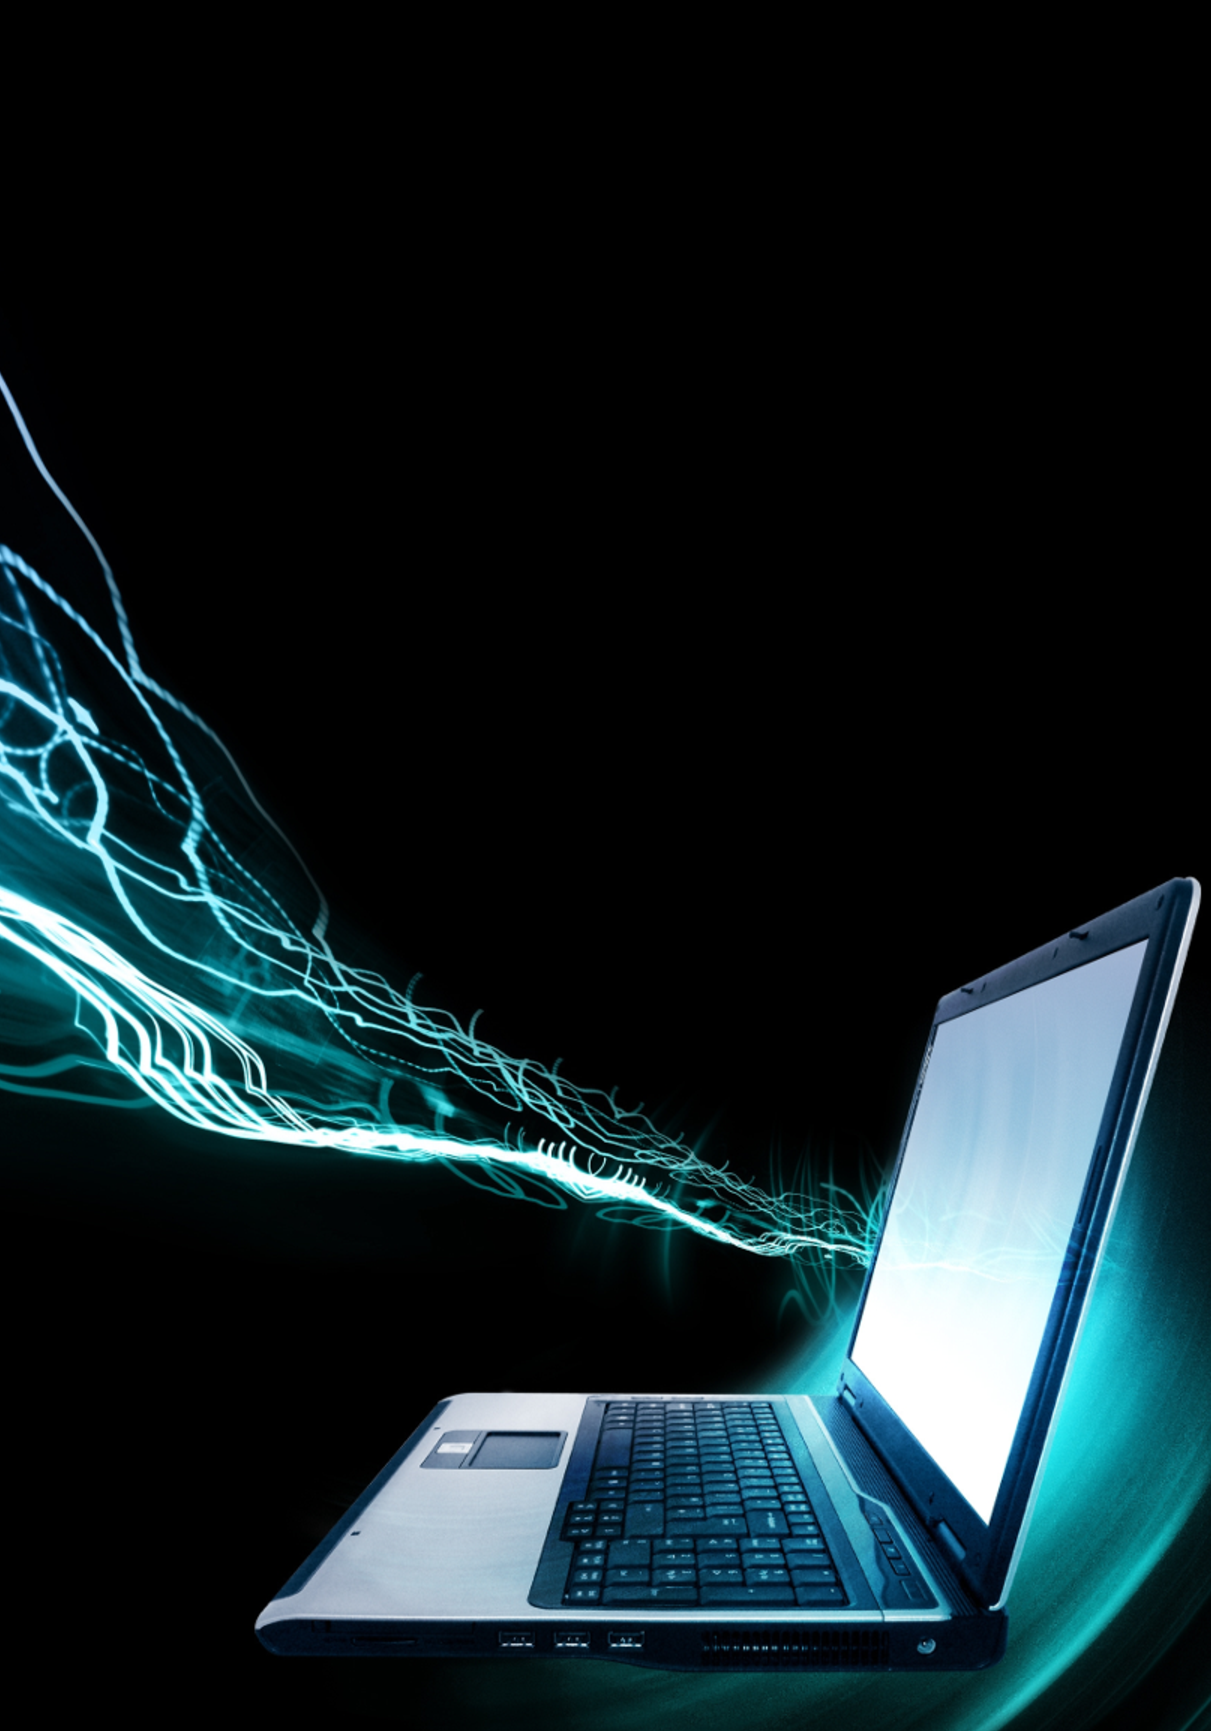
\includegraphics[width=\paperwidth]{background}}; % Background image
\draw[anchor=north] (midpoint) node [fill=ocre!30!white,fill opacity=0.6,text
opacity=1,inner
sep=1cm]{\Huge\centering\bfseries\sffamily\parbox[c][][t]{\paperwidth}{\centering
    {\color{white} Distributed Hosting}\\[15pt] % Book title
{\Large {\color{white} A Blockchain Based Distributed Hosting Engine}}\\[20pt] % Subtitle
{\normalsize {\color{white} Alex Oberhauser, Stavros Champilomatis and Maria Efthimiadou}}}}; % Author name
\end{tikzpicture}};
\end{tikzpicture}
\vfill
\endgroup

%------------------------------------------------------------------------------
%	COPYRIGHT PAGE
%------------------------------------------------------------------------------

\newpage
~\vfill
\thispagestyle{empty}

\noindent Copyright \copyright\ 2015 Alex Oberhauser, Stavros Champilomatis and Maria Efthimiadou\\ % Copyright notice

\noindent \textsc{Published by the \textit{Distributed Hosting} team}\\ % Publisher

\noindent \textsc{http://blackgate.networld.to}\\ % URL

\noindent This work is licensed under the Creative Commons Attribution 4.0 International License. To view this license visit \url{http://creativecommons.org/licenses/by/4.0/}.\\ % License information

\noindent \textit{First released, March 2015} % Printing/edition date

%------------------------------------------------------------------------------
%	TABLE OF CONTENTS
%------------------------------------------------------------------------------

\chapterimage{chapter_head_1.pdf} % Table of contents heading image

\pagestyle{empty} % No headers

\tableofcontents % Print the table of contents itself

\cleardoublepage % Forces the first chapter to start on an odd page so it's on the right

\pagestyle{fancy} % Print headers again

%------------------------------------------------------------------------------
%	PART
%------------------------------------------------------------------------------
\part{Overview}

%------------------------------------------------------------------------------
%	CHAPTER 1
%------------------------------------------------------------------------------

\chapterimage{chapter_head_2.pdf} % Chapter heading image

\chapter{Introduction}
% -*- root: ../distributed_hosting_whitepaper.tex -*-

This part gives a motivation and a general overview about the
\textit{Distributed Hosting Engine}. It introduces some concepts that will be
explained in more detail in the next part. If you are looking for a detailed specification you can directly go to Part \ref{part:specifications}.

\section{Hosting Paradigm Shift}\index{Hosting Paradigm Shift}

This whitepaper specifies a new protocol and blockchain that has
the potential to change the current hosting paradigm. Instead of retrieving
pages from a specific location, they are hosted directly on end-user
devices. The distributed hosting algorithm and protocol, specified here, takes
care of the optimal location for each page. By taking into account different
metrics, like response times, availability and/or relevance, the perfect place
for each page will be found after some time. This not only increases the
performance for single page accesses, but reduced also network load and hence
increases the overall network health.

Additional to the increased performance, the underlying blockchain assures the
correctness and validity of each page, also, or especially, if hosted by a
random node in the network. This validation mechanism is then used to create a
reputation system, allowing blocking of malicious nodes that have a reputation
score that is lower than a threshold value.

This mechanism, together with the page distribution algorithm, makes the
network self-managing, self-healing and robust against changes.

By design the \textit{Distributed Hosting Engine} is censorship resistance,
but only under the assumption that there are enough nodes that are willing to
host the page. This moves responsibility what could be hosted from a central
authority to the collective.

From a commercial point of view the here proposed approach allows the creation
of an interoperable hosting ecosystem. Each hosting provider acts as clone and
has no direct access to the page, but can support the user with additional
(paid or free) services and hosting space. By design a switch from one
hosting provider to another one does not affect the hosting of the page, nor
the page itself. Technical there is not even a migration happening, only a
switch from one page creation tool to another one.

\section{Use Cases}\index{Use Cases}

\textbf{TODO:} Explains here different use cases based on user stories of Jane
and John Doe.


\chapter{Empowering Technology}
% -*- root: ../distributed_hosting_whitepaper.tex -*-

This chapter explains the technologies that make the \textit{Distributed
Hosting Engine} possible. Most notable the concept of \textit{Blockchains} for
the distributed management and self-organization of pages and \textit{Tor
Hidden Services} that not only protect the privacy of all involved parties,
but that also allows to host pages behind NATs and Firewalls.

\section{Blockchain}\index{Blockchain}

\textit{Blockchain} is a rather new concept, with a lot of potential. A
\textit{Blockchain} is a distribute ledgers that prevents double spending without a central authority. The first time the \textit{Blockchain} was mentioned and implemented was for Bitcoin \cite{nakamoto2008bitcoin}.

\section{Tor Hidden Services}\index{Tor Hidden Services}

Tor hidden services are generally used to host pages anonymously and protect
visitors and hosters alike. In the scope of this whitepaper tor hidden
services are used to enable hosting from everywhere, no matter if the device
is behind a NAT or a Firewall. This allows to host pages from public wireless
hotspots, from the office or from home. Without the possibility to abstract
away from public accessible IPs and the capability to circumvent Firewalls it
would not be possible to develop real distributed hosting on end-user devices.


\chapter{Ecosystem}
% -*- root: ../distributed_hosting_whitepaper.tex -*-

\section{Hosting Provider}\index{Hosting Provider}

\textbf{TODO:} \textit{Explain here the role change of hosting providers. For
example: A hosting provider does provide service on top of the blockchain,
like page generators and frontends for page publications and updates. If a
hosting provider decides to host a page, it is only one clone out of many
without special role.}
\newline

By introducing the \textit{Distributed Hosting Engine} the role of hosting
providers will change. Instead of being the only entity that hosts an instance
of a page, they will be part of an overall network of hosters. The hosting
responsibility is shared between always-on devices, like servers and
partially-on devices, like laptops or desktop computers. Additional a single
hosting provider will not be able to control the distribution of the page,
because that is determined by the collective of nodes in the network. That
said, hosting providers are playing an important role in the overall
ecosystem. They not only guarantee uptime of pages by hosting them 24/7, but
can also provide additional services that abstract away from the underlying
blockchain and page development. Especially the former point is important in
the early stage of the network and/or when a new page joins the network. A
bigger network with pages that had time to distribute in an optimal way makes
dedicated hosting servers unnecessary.

\section{Complementary Services}\index{Complementary Services}

\textbf{TODO:} \textit{Figure out what alternatives services could be provided
by the ecosystem. This includes also new business ideas for new types of
startups.}
\newline

\begin{description}
\item[Hosting Space] As mentioned in the previous section, in the early stage
there is a need for 24/7 online hosting servers in order to guarantee uptime.
These \textit{Clones} are not different than any other clone, except that they
are always online.
\item[Page Generation] The countless simple page generation services that
exists today can be used to support non-technical users to host their pages.
\item[Host Wallets] Like Bitcoin Wallets this \textit{Host Wallets} manage all
pages related to one users. Not really recommended for security reasons,
because private keys are controlled by the \textit{Host Wallet} provider.
\end{description}



%------------------------------------------------------------------------------
%	PART
%------------------------------------------------------------------------------
\part{Specifications}\label{part:specifications}

%------------------------------------------------------------------------------
%	CHAPTER 2
%------------------------------------------------------------------------------

\chapterimage{chapter_head_2.pdf} % Chapter heading image

\chapter{Blockchain Specification}

\section{Transaction Definition}\index{Transaction Definition}
% -*- root: ../distributed_hosting_whitepaper.tex -*-

This section defines transactions and their relationship to each other and to
external data. It also defines a (de-)serialization format to and
from the binary format that is transferred over the wire. In Figure
\ref{fig:transactions} a chain of transactions, with relevant fields, is
shown. This example includes three hosts that have cloned the page and in total
three updates.

\begin{figure}[htp]
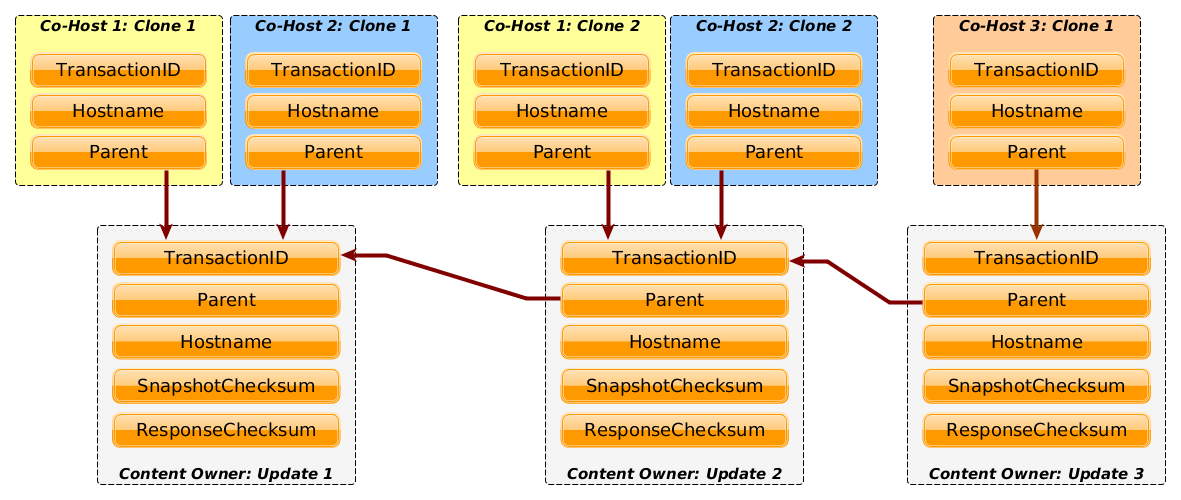
\includegraphics[width=\textwidth]{transactions.png}
\label{fig:transactions}
\caption{Transaction chain example for one page.}
\end{figure}

\subsection{UPDATE Transaction Definition}

Update transactions can only be created by the page creator. Additional to the
proof of ownership they also include a reference to the new content, with
related checksums.

\begin{table}[ht]
  \centering
  \begin{tabular}{|g|p{10cm}|}
    \hline
    \multicolumn{2}{|c|}{\textbf{TRANSACTION HEADER}}\\
    \hline
    \textbf{TransactionID} & Double SHA256 hash of this transaction.\\
    \hline
    \textbf{Parent} & The previous update \textit{TransactionID}\\
    \hline
    \textbf{ScriptSig} & \textbf{TODO Future Work:} Proof here ownernship of
    the hostname and all requirements that come with this update.\\
    \hline
    \textbf{Hostname} & The tor hidden service onion hostname of this page.
    Tor hidden services are needed to be able to host page behind firewalls
    and NATs. Additional they protect the identity of the content owner and
    more importantly of clone hosts.\\
    \hline
    \multicolumn{2}{|c|}{\textbf{CONTENT SECTION}}\\
    \hline
    \textbf{Snapshot} & The hash value of the content. This hash value is used
    to find all peers in the Distributed Hash Table (DHT) that share currently
    this snapshot. The DHT is bootstrapped by using all active hostname in the
    blockchain. For increased compatibility the MAGNET URI scheme is used.\\
    \hline
    \textbf{SnapshotChecksum} & Checksum of the Snapshot content, used to
    verify the downloaded data.\\
    \hline
    \textbf{ResponseChecksum} & Checksums for all endpoints of this page.
    Makes each page verifiable and hence could be served by a random node. If
    the returned content does not match the here checksum the response is
    invalid.\\
    \hline
    \textbf{Flags} & \textbf{TODO Future Work:} Could be used for
    differentiation between incremental and full updates, but also indicating
    that this page is not hosted anymore and could be deleted.\\
    \hline
  \end{tabular}
\end{table}

\subsection{CLONE Transaction Definition}

\textbf{TODO:} This transaction can be merge with the UPDATE transaction. They
do not differ too  much, except that they have different Flags content and
that the CLONE transaction does not include all fields.

Clone transactions are created and propagated by all hosts that start hosting
a page or if they receive a new update transaction. This transactions always
link back to exactly one update transaction.

\begin{table}[ht]
  \centering
  \begin{tabular}{|g|p{10cm}|}
    \hline
    \textbf{TransactionID} & Double SHA256 hash of this transaction.\\
    \hline
    \textbf{Parent} & The previous update \textit{TransactionID}\\
    \hline
    \textbf{ScriptSig} & \textbf{TODO Future Work:} Proof here ownernship of
    the hostname and all requirements that come with this update.\\
    \hline
    \textbf{Hostname} & The tor hidden service onion hostname of this page.
    Tor hidden services are needed to be able to host page behind firewalls
    and NATs. Additional they protect the identity of the content owner and
    more importantly of clone hosts.\\
    \hline
    \textbf{Flags} & Possible values are: \textit{CLONE} when new update was
    received or \textit{PURGE} if the page is not hosted anymore.\\
    \hline
  \end{tabular}
\end{table}


\section{Block Definition}\index{Block Definition}

\section{Mining Process}\index{Mining Process}
% -*- root: ../distributed_hosting_whitepaper.tex -*-

\textbf{Note:} \textit{This section is work in progress. The resulting
description is a first naive solution. Currently in discussion are multi-
entity ownerships and a consensus network between this small group of page
owners, e.g. with Practical Byzantine Fault Tolerance (PBFT)
\cite{castro1999practical}.}

By definition each page in the hosting space has an own blockchain. In the
\textit{Genesis Block} the \textit{Content Creator} proofs ownership of this
blockchain and hence the related page. The assumption here is that only the
\textit{Content Creator} can update the page and that (s)he is the only entity
that has not intention to compromise the own page.


%----------------------------------------------------------------------------------------
%	CHAPTER 3
%----------------------------------------------------------------------------------------
\chapter{Protocol Specification}

In Figure \ref{fig:data_cloud_blockchain} the relationship between the page
content (html, css, javascript, images...), in the middle cloud, the data
(above) and blockchain overlay network (below) is shown. The network that
manages the page content has not to be the same as the blockchain network, but
they maybe nearly identical or overlapping. The page content is not part of
the blockchain, but referenced from it. This allows to have no page content
size limit and the data exchange could be optimized.

\begin{figure}[htp]
\centering
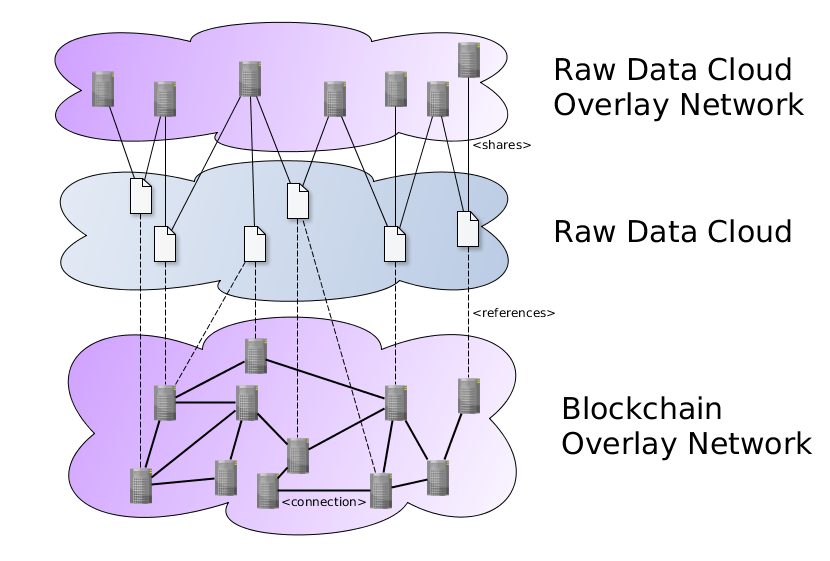
\includegraphics[width=0.75\textwidth]{pictures/data_cloud_blockchain.png}
\caption{Relationship between blockchain and page content from a network
perspective.}
\label{fig:data_cloud_blockchain}
\index{Overlay Networks Figure}
\end{figure}


\section{Blockchain Overlay Network}\index{Blockchain Overlay Network}
\section{Data Overlay Network}\index{Data Overlay Network}
\section{Hosting Algorithm}\index{Hosting Algorithm}

%----------------------------------------------------------------------------------------
%	PART
%----------------------------------------------------------------------------------------
\part{Appendix}

%----------------------------------------------------------------------------------------
%	BIBLIOGRAPHY
%----------------------------------------------------------------------------------------

\chapter*{Bibliography}
\addcontentsline{toc}{chapter}{\textcolor{ocre}{Bibliography}}
%\section*{Books}
%\addcontentsline{toc}{section}{Books}
%\printbibliography[heading=bibempty,type=book]
%\section*{Articles}
%\addcontentsline{toc}{section}{Articles}
%\addcontentsline{toc}{section}{Articles}
%\printbibliography[heading=bibempty,type=article]
%\nocite{*}
\printbibliography[heading=bibempty]

%----------------------------------------------------------------------------------------
%	INDEX
%----------------------------------------------------------------------------------------

\cleardoublepage
\phantomsection
\setlength{\columnsep}{0.75cm}
\addcontentsline{toc}{chapter}{\textcolor{ocre}{Index}}
\printindex

%----------------------------------------------------------------------------------------

\end{document}
